\documentclass[11pt,a4paper]{article}
\usepackage[margin=19mm,top=20mm,bottom=20mm]{geometry}
\usepackage{amsmath,amssymb,graphicx,array,fancyhdr,lastpage,textcomp,fancyvrb}
\usepackage{fontspec}
\usepackage[hidelinks]{hyperref}
\setmainfont{texgyreheros-regular.otf}[BoldFont=texgyreheros-bold.otf,ItalicFont=texgyreheros-italic.otf,BoldItalicFont=texgyreheros-bolditalic.otf]
\setmonofont{lmmono10-regular.otf}
\setlength{\parindent}{0pt}\setlength{\parskip}{5pt}
\setlength{\headheight}{14pt}
\pagestyle{fancy}\fancyhf{}
\renewcommand{\headrulewidth}{0.3pt}\renewcommand{\footrulewidth}{0.3pt}
\fancyfoot[L]{\footnotesize by paper.shrit.in\quad |\quad normal}
\fancyfoot[R]{\footnotesize Page \thepage\ of \pageref{LastPage}}
\begin{document}
\fancyhead[L]{\small Digital Systems and Computer Organization}\fancyhead[R]{\small Set B: Original}
{\LARGE\bfseries Worked Solutions}\par{\large Digital Systems and Computer Organization}\par\textbf{Set B: Original | CSE Semester 3}\par
Companion to \texttt{dsco-original.pdf}. Question numbers match that paper. Equivalent correct methods are acceptable. These are independent worked solutions, not an official university marking scheme.\par\medskip\hrule\medskip
Questions 1--5: MCQ answer key, 1 mark each (5 marks total). Questions 6 onward: theory solutions (25 marks total).\par
\noindent\begin{minipage}{\linewidth}\subsection*{1. K-map cell count}
\textbf{Correct option: (C).} There is one cell per input combination, so $2^4=16$ cells.
\end{minipage}\par\medskip
\noindent\begin{minipage}{\linewidth}\subsection*{2. K-map adjacency}
\textbf{Correct option: (A).} Gray-code ordering makes adjacent cells differ in exactly one variable.
\end{minipage}\par\medskip
\noindent\begin{minipage}{\linewidth}\subsection*{3. SOP grouping}
\textbf{Correct option: (D).} Groups contain a power of two cells; 8 is the only power of two listed.
\end{minipage}\par\medskip
\noindent\begin{minipage}{\linewidth}\subsection*{4. Function reduction}
\textbf{Correct option: (B).} Every listed minterm has $B=D$. Thus $F=\neg B\neg D+BD$, independent of A and C.
\end{minipage}\par\medskip
\noindent\begin{minipage}{\linewidth}\subsection*{5. NAND inverter}
\textbf{Correct option: (C).} Connecting both inputs to X gives $\neg(X\cdot X)=\neg X$.
\end{minipage}\par\medskip
\noindent\begin{minipage}{\linewidth}\subsection*{6. Signed results and overflow}
\begin{center}\renewcommand{\arraystretch}{1.2}\begin{tabular}{lllll}\hline Operation & Binary addition & Result & Interpretation & Overflow\\\hline
11+7 & 01011 + 00111 & 10010 & -14 & Yes\\
-9+5 & 10111 + 00101 & 11100 & -4 & No\\
6-13 & 00110 + 10011 & 11001 & -7 & No\\\hline\end{tabular}\end{center}Only the true result 18 is outside $[-16,15]$. For subtraction, 13 is 01101 and its two's-complement negative is 10011. A carry out by itself is not the signed-overflow flag.
\end{minipage}\par\medskip
\noindent\begin{minipage}{\linewidth}\subsection*{7. MUX realization}
With A and B as select bits (A most significant), $AB=00,01,10,11$ produces $C,\bar C,\bar C,C$, respectively. Thus $\boxed{I_0=C,\ I_1=\bar C,\ I_2=\bar C,\ I_3=C}$. One inverter supplies both complemented-C inputs.\begin{center}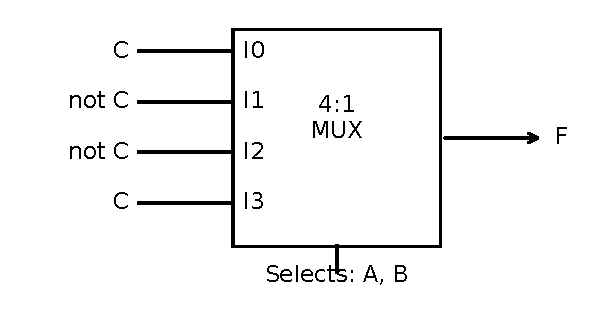
\includegraphics[width=.65\linewidth]{figures/mux.pdf}\end{center}
\end{minipage}\par\medskip
\noindent\begin{minipage}{\linewidth}\subsection*{8. Enabled two-bit synchronous counter}
\begin{center}\renewcommand{\arraystretch}{1.2}\begin{tabular}{lll}\hline Present $q_1q_0$ & Next when E=0 & Next when E=1\\\hline
00 & 00 & 01\\
01 & 01 & 10\\
10 & 10 & 11\\
11 & 11 & 00\\\hline\end{tabular}\end{center}
Use the T excitation equation $T_i=q_i\oplus q_i^+$. The low bit toggles exactly when E=1; the high bit toggles exactly when E=1 and the current low bit is 1.
\[\boxed{T_0=E,\qquad T_1=Eq_0}.\]
Feed E directly to $T_0$ and an AND of E and $q_0$ to $T_1$. The clock is common.
\begin{center}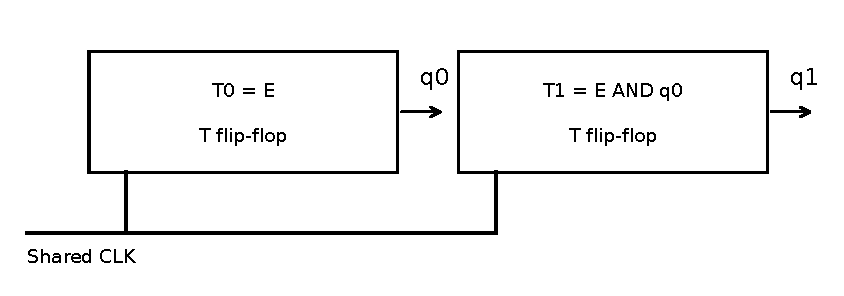
\includegraphics[width=.85\linewidth]{figures/counter2.pdf}\end{center}
\end{minipage}\par\medskip
\noindent\begin{minipage}{\linewidth}\subsection*{9. Four-bit ring counter}
\VerbatimInput[fontsize=\footnotesize]{code/ring4.v}
On a positive clock edge with reset high, q becomes 0001. With reset low, successive states are 0010, 0100, 1000 and 0001. Concatenation moves bits 2:0 upward and puts old bit 3 into bit 0. Nonblocking assignments model sequential storage.
\end{minipage}\par\medskip
\noindent\begin{minipage}{\linewidth}\subsection*{10. Ripple delay and decoded glitches}
A ripple counter clocks stage 0 from the external clock and later stages from preceding flip-flop outputs. Propagation delays accumulate, so several output bits do not change simultaneously. During a transition such as 0111 to 1000, a decoder may briefly recognize an intermediate pattern. A synchronous counter drives all flip-flops from one shared clock and computes excitation logic from the old state. It avoids stage-by-stage clock ripple, although real output skew and combinational delays still require proper timing design.
\end{minipage}\par\medskip
\noindent\begin{minipage}{\linewidth}\subsection*{11. Two-bit magnitude comparator}

Let $e_i=a_i\operatorname{XNOR}b_i$. Then
\[\boxed{G=a_1\bar b_1+e_1a_0\bar b_0},\qquad
\boxed{E_q=e_1e_0},\qquad
\boxed{L=\bar a_1b_1+e_1\bar a_0b_0}.\]
The upper bit decides unless equal; only then does the lower bit decide. Use XNOR gates for $e_1,e_0$, inverters for complements, AND gates for product terms and OR gates to combine them. The figure gives the G network. Swap a and b for L, and AND the two XNOR outputs for $E_q$.
\begin{center}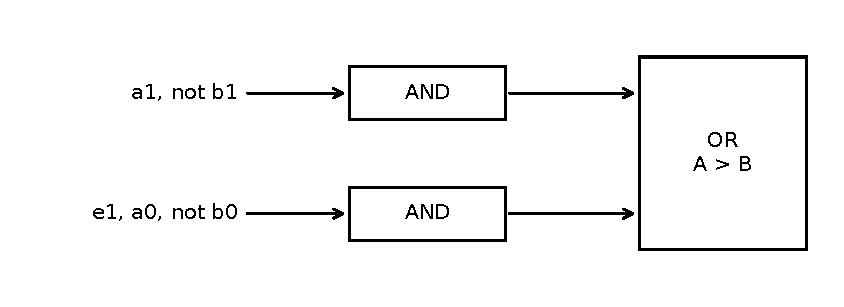
\includegraphics[width=.85\linewidth]{figures/comparator2.pdf}\end{center}For A=10 and B=01, $e_1=0$, $a_1\bar b_1=1$, so $\boxed{G=1,E_q=0,L=0}$.
\end{minipage}\par\medskip
\noindent\begin{minipage}{\linewidth}\subsection*{12. Memory capacity and addresses}

4 KiB $=4096$ bytes. Each 32-bit word occupies 4 bytes:
\[\text{words}=4096/4=\boxed{1024},\qquad
\text{byte-select bits}=\log_2(4096)=\boxed{12}.\]
The word at 0x1000 occupies 0x1000, 0x1001, 0x1002 and 0x1003. The next word starts at 0x1004. The 12 bits select an offset within the 4 KiB block; the full system may use more address bits to place that block at base 0x1000. Endianness changes byte significance, not these occupied addresses.
\end{minipage}\par\medskip
\noindent\begin{minipage}{\linewidth}\subsection*{13. Memory read and write}

For a read: place the target address in MAR, assert the read control signal, wait until the memory interface indicates valid data, and latch the returned value into MDR. Transfer MDR to the destination register as required.

For a write: place the target address in MAR and outgoing data in MDR, assert write with the required timing, and wait for completion. Read moves data from memory to MDR; write moves data from MDR to memory. MAR selects the location in both cases.
\end{minipage}\par\medskip

\end{document}
